% ============================================================================
% Korean Resume Template with Profile Photo
% Based on Saramin/JobKorea Standard Format
% Engine: XeLaTeX + kotex
% ============================================================================

\documentclass[a4paper, 10pt]{article}

% ============================================================================
% PACKAGES
% ============================================================================

\usepackage{kotex}
\usepackage{fontspec}
\usepackage[a4paper, top=15mm, bottom=15mm, left=20mm, right=20mm]{geometry}
\usepackage{tabularx}
\usepackage{array}
\usepackage{colortbl}
\usepackage{graphicx}
\usepackage{xcolor}
\usepackage[hidelinks]{hyperref}
\usepackage{calc}

% ============================================================================
% FONTS
% ============================================================================

\setmainfont{Malgun Gothic}[Script=Hangul, Language=Korean]
\setmainhangulfont{Malgun Gothic}
\setsanshangulfont{Malgun Gothic}

% ============================================================================
% PAGE SETUP
% ============================================================================

\pagestyle{empty}
\setlength{\parindent}{0pt}
\setlength{\parskip}{0pt}
\setlength{\baselineskip}{0.95\baselineskip}
\renewcommand{\arraystretch}{0.95}

% ============================================================================
% COLORS
% ============================================================================

\definecolor{navyblue}{RGB}{31, 73, 125}
\definecolor{lightblue}{RGB}{220, 230, 242}
\definecolor{darkgray}{RGB}{80, 80, 80}

% ============================================================================
% CUSTOM COMMANDS
% ============================================================================

\newcommand{\resumesection}[1]{%
  \vspace{3pt}
  \noindent
  \begin{tabularx}{\textwidth}{|X|}
    \hline
    \rowcolor{navyblue}
    \textcolor{white}{\large\textbf{#1}} \\
    \hline
  \end{tabularx}
  \vspace{1pt}
}

\newcommand{\labelcell}[1]{%
  \cellcolor{lightblue}\textbf{#1}
}

\newcommand{\headercell}[1]{%
  \cellcolor{navyblue}\textcolor{white}{\textbf{#1}}
}

% ============================================================================
% DOCUMENT START
% ============================================================================

\begin{document}

% ============================================================================
% HEADER WITH NAME AND PHOTO
% ============================================================================

\begin{minipage}[t]{0.72\textwidth}
  \vspace{0pt}
  {\fontsize{28}{28}\selectfont\textbf{\textcolor{navyblue}{조\ 동\ 휘}}}

  \vspace{6pt}

  {\large CHOI DONGHWI}

  \vspace{8pt}

  {\color{darkgray}\small
  나이: 26세(1999.07.11) | 성별: 남 | 경력: 1년 이상 | 소프트웨어 개발\\
  연락처: 010-8699-1510 | 이메일: donghwi0711@icloud.com \\
  GitHub: \href{https://github.com/nobrain711}{github.com/nobrain711}
  }
\end{minipage}
\begin{minipage}[t]{0.25\textwidth}
  \vspace{0pt}
  \begin{center}
    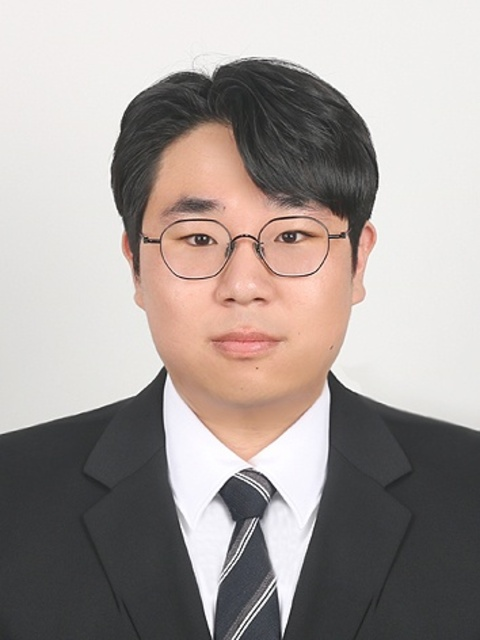
\includegraphics[width=3.5cm, height=4.5cm, keepaspectratio]{images/profile/증명사진.jpg}

    {\tiny\color{gray}(3×4cm)}
  \end{center}
\end{minipage}

\vspace{8pt}

% ============================================================================
% EDUCATION
% ============================================================================

\resumesection{학\ 력\ 사\ 항}

\begin{tabularx}{\textwidth}{|p{2.8cm}|p{3.5cm}|X|p{1.5cm}|}
  \hline
  \headercell{재학기간} & \headercell{학교명 및 전공} & \headercell{학점} & \headercell{비고} \\
  \hline
  2021.03--2024.02 & 영남이공대학교 컴퓨터공학과 & 3.75/4.5 & 졸업 \\
  \hline
  2016.03--2019.02 & 춘천기계공업고등학교 자동차과 & -- & 졸업 \\
  \hline
\end{tabularx}

% ============================================================================
% WORK EXPERIENCE
% ============================================================================

\resumesection{경\ 력\ 사\ 항}

\begin{tabularx}{\textwidth}{|p{2.8cm}|p{3cm}|p{2.2cm}|X|}
  \hline
  \headercell{근무기간} & \headercell{근무회사} & \headercell{직위} & \headercell{담당직무} \\
  \hline
  2024.04--2025.01 & (주)토마토 & 소프트웨어 엔지니어 & AWS EC2 금융 시스템 인프라 구축, Windows Server 환경 설정, SOP 작성 \\
  \hline
\end{tabularx}

% ============================================================================
% LANGUAGE
% ============================================================================

\resumesection{어\ 학}

\begin{tabularx}{\textwidth}{|X|p{2.5cm}|p{2.5cm}|}
  \hline
  \headercell{시험명} & \headercell{점수/등급} & \headercell{취득일} \\
  \hline
  TOEIC & 920점 & 2023.05.14 \\
  \hline
  OPIc & IM2 & 2023.09.10 \\
  \hline
\end{tabularx}

% ============================================================================
% EDUCATION/TRAINING
% ============================================================================

\resumesection{교\ 육\ 및\ 연\ 수}

\begin{tabularx}{\textwidth}{|p{2.8cm}|X|p{3.5cm}|}
  \hline
  \headercell{기간} & \headercell{과정명} & \headercell{기관} \\
  \hline
  2025.07--2025.08 & Czech IT Out Summer School 2025 & University of Hradec Kralove \\
  \hline
  2026.01--2026.07 & SK 네트웍스 Family AI 캠프 & 플레이데이터 \\
  \hline
\end{tabularx}

% ============================================================================
% ACTIVITIES
% ============================================================================

\resumesection{활\ 동}

\begin{tabularx}{\textwidth}{|p{2.8cm}|X|p{3.5cm}|}
  \hline
  \headercell{기간} & \headercell{활동 내용} & \headercell{기관} \\
  \hline
  2024.03--2024.12 & 멋쟁이사자처럼 at 명지대(서울) & 멋쟁이사자처럼 \\
  \hline
  2023.03--2026.02 & 명지대 중앙 자전거 동아리 굴렁쇠 & 명지대학교 \\
  \hline
\end{tabularx}

% ============================================================================
% AWARDS
% ============================================================================

\resumesection{수\ 상}

\begin{tabularx}{\textwidth}{|p{2.8cm}|X|p{3.5cm}|}
  \hline
  \headercell{기간} & \headercell{상장 내용} & \headercell{기관} \\
  \hline
  2024.10 & 멋쟁이사자처럼 명지톤 대상 & 멋쟁이사자처럼 \\
  \hline
  2021.11 & 2021 Denmark X CO.Ad AD Festival 최우수상 & 동원 F\&B \\
  \hline
\end{tabularx}

% ============================================================================
% CERTIFICATIONS
% ============================================================================

\resumesection{자\ 격\ 증}

\begin{tabularx}{\textwidth}{|X|p{4.5cm}|}
  \hline
  \headercell{자격증명} & \headercell{발급기관} \\
  \hline
  정보처리기사 & 한국산업인력공단 \\
  \hline
  SQLD & 한국데이터산업진흥원 \\
  \hline
\end{tabularx}

% ============================================================================
% SKILLS
% ============================================================================

\resumesection{기\ 술\ 및\ 능\ 력}

\begin{tabularx}{\textwidth}{|p{2.8cm}|X|}
  \hline
  \headercell{프로그래밍} & Python, JavaScript/TypeScript, SQL, Bash \\
  \hline
  \headercell{웹 프레임워크} & FastAPI, Django, React, Express.js \\
  \hline
  \headercell{데이터베이스} & PostgreSQL, MySQL, MongoDB, Redis \\
  \hline
  \headercell{클라우드/DevOps} & AWS (EC2, S3, RDS), Docker, GitHub Actions, Kubernetes \\
  \hline
  \headercell{개발 도구} & Git, VS Code, Postman, Jupyter Notebook, Notion \\
  \hline
\end{tabularx}

\end{document}
